\documentclass[12pt]{article}
\usepackage{latexsym,amssymb,amsmath} % for \Box, \mathbb, split, etc.
% \usepackage[]{showkeys} % shows label names
\usepackage{cite} % sorts citation numbers appropriately
\usepackage{path}
\usepackage{url}
\usepackage{verbatim}
\usepackage{graphicx}
\usepackage{array}
\usepackage{multirow}

% horizontal margins: 1.0 + 6.5 + 1.0 = 8.5
\setlength{\oddsidemargin}{0.0in}
\setlength{\textwidth}{6.5in}
% vertical margins: 1.0 + 9.0 + 1.0 = 11.0
\setlength{\topmargin}{0.0in}
\setlength{\headheight}{12pt}
\setlength{\headsep}{13pt}
\setlength{\textheight}{625pt}
\setlength{\footskip}{24pt}

\renewcommand{\textfraction}{0.10}
\renewcommand{\topfraction}{0.85}
\renewcommand{\bottomfraction}{0.85}
\renewcommand{\floatpagefraction}{0.90}
\usepackage{graphicx}
\usepackage{wrapfig}
\usepackage{lscape}
\usepackage{rotating}
\usepackage{epstopdf}
\makeatletter
\setlength{\arraycolsep}{2\p@} % make spaces around "=" in eqnarray smaller
\makeatother

% change equation, table, figure numbers to be counted inside a section:
\numberwithin{equation}{section}
\numberwithin{table}{section}
\numberwithin{figure}{section}

% begin of personal macros
\newcommand{\half}{{\textstyle \frac{1}{2}}}
\newcommand{\eps}{\varepsilon}
\newcommand{\myth}{\vartheta}
\newcommand{\myphi}{\varphi}
\usepackage[utf8]{inputenc}

% Default fixed font does not support bold face
\DeclareFixedFont{\ttb}{T1}{txtt}{bx}{n}{8} % for bold
\DeclareFixedFont{\ttm}{T1}{txtt}{m}{n}{8}  % for normal

% Custom colors
\usepackage{color}
\definecolor{deepblue}{rgb}{0,0,0.5}
\definecolor{deepred}{rgb}{0.6,0,0}
\definecolor{deepgreen}{rgb}{0,0.5,0}
\definecolor{backcolour}{rgb}{0.96,0.96,0.96}

\usepackage{listings}

% cpp style for highlighting
\newcommand\cppstyle{\lstset{
		language=C++,
        basicstyle=\tiny\ttfamily,
		keywordstyle=\color{blue}\ttfamily,
		stringstyle=\color{red}\ttfamily,
		commentstyle=\color{green}\ttfamily,
		morecomment=[l][\color{magenta}]{\#},
		frame=tb,                         % Any extra options here
showstringspaces=false,            % 
backgroundcolor=\color{backcolour}
}}


% cpp environment
\lstnewenvironment{cpp}[1][]
{
	\cppstyle
	\lstset{#1}
}
{}

% cpp for external files
\newcommand\cppexternal[2][]{{
		\cppstyle
		\lstinputlisting[#1]{#2}}}

% cpp for inline
\newcommand\cppinline[1]{{\cppstyle\lstinline!#1!}}

\newcommand{\IN}{\mathbb{N}}
\newcommand{\IZ}{\mathbb{Z}}
\newcommand{\IQ}{\mathbb{Q}}
\newcommand{\IR}{\mathbb{R}}
\newcommand{\IC}{\mathbb{C}}
\newcommand{\Real}[1]{\mathrm{Re}\left({#1}\right)}
\newcommand{\Imag}[1]{\mathrm{Im}\left({#1}\right)}
\usepackage{booktabs}
\usepackage{caption}
\usepackage{float}
\usepackage{titlesec}
\usepackage{capt-of}
%dashed line
\usepackage{array}
\usepackage{arydshln}
\setlength\dashlinedash{0.2pt}
\setlength\dashlinegap{1.5pt}
\setlength\arrayrulewidth{0.3pt}

%Widows & Orphans & Penalties

\widowpenalty500
\clubpenalty500
\clubpenalty=9996
\exhyphenpenalty=50 %for line-breaking at an explicit hyphen
\brokenpenalty=4991
\predisplaypenalty=10000
\postdisplaypenalty=1549
\displaywidowpenalty=1602
\floatingpenalty = 20000
\usepackage[T1]{fontenc}
\usepackage{fontspec}
\setmainfont[Scale=0.85, Ligatures={Required,Common,Contextual,TeX}]{TeX Gyre Schola} % Incredible font inside latex


\newcommand{\norm}[2]{\|{#1}\|_{{}_{#2}}}
\newcommand{\abs}[1]{\left|{#1}\right|}
\newcommand{\ip}[2]{\left\langle {#1}, {#2} \right\rangle}
\newcommand{\der}[2]{\frac{\partial {#1}}{\partial {#2}}}
\newcommand{\dder}[2]{\frac{\partial^2 {#1}}{\partial {#2}^2}}
\usepackage{enumitem}
\newcommand{\nn}{\mathbf{n}}
\newcommand{\xx}{\mathbf{x}}
\newcommand{\uu}{\mathbf{u}}
\usepackage{tikz}
\usetikzlibrary{arrows}
\usetikzlibrary{positioning}
\usepackage{titlesec}
\newcommand{\junk}[1]{{}}
\usepackage{sectsty}
\usepackage{xcolor}

\newcommand\MyBox[2]{
	\fbox{\lower0.75cm
		\vbox to 1.7cm{\vfil
			\hbox to 1.7cm{\hfil\parbox{1.4cm}{#1\\#2}\hfil}
			\vfil}%
	}%
}

\makeatletter
\renewcommand*\env@matrix[1][\arraystretch]{%
	\edef\arraystretch{#1}%
	\hskip -\arraycolsep
	\let\@ifnextchar\new@ifnextchar
	\array{*\c@MaxMatrixCols c}}
\makeatother

\makeatletter
\renewcommand*\env@matrix[1][*\c@MaxMatrixCols c]{%
	\hskip -\arraycolsep
	\let\@ifnextchar\new@ifnextchar
	\array{#1}}
\makeatother

\definecolor{darkblue}{rgb}{0,0,0.4}
\usepackage[colorlinks = true,
linkcolor = darkblue,
urlcolor  = darkblue,
citecolor = darkblue,
anchorcolor = darkblue]{hyperref}
% set two lengths for the includegraphics commands used to import the plots:
\newlength{\fwtwo} \setlength{\fwtwo}{0.45\textwidth}
% end of personal macros

\begin{document}
\DeclareGraphicsExtensions{.jpg}

\begin{center}
\textsc{\Huge Multi-core Programming} \\[2pt]
	\textsc{\Large Assignment 4}\\
	\vspace{0.5cm}
  Ali Gholami \\[6pt]
  Department of Computer Engineering \& Information Technology\\
  Amirkabir University of Technology  \\[6pt]
  \def\UrlFont{\em}
  \url{https://aligholamee.github.io}\\
\href{mailto:aligholami7596@gmail.com}{\textit{aligholami7596@gmail.com}}
\end{center}

\begin{abstract}
Graphics processing units (GPUs) originally designed for computer video cards have emerged as the most powerful chip in a high-performance workstation. Unlike multicore CPU architectures, which currently ship with two or four cores, GPU architectures are “manycore” with hundreds of cores capable of running thousands of threads in parallel. NVIDIA’s CUDA is a co-evolved hardware-software architecture that enables high-performance computing developers to harness the tremendous computational power and memory bandwidth of the GPU in a familiar programming environment - the C programming language. In this report, we'll analyze the basic architectural characteristics of Nvidia GPUs.
\end{abstract} 

\subparagraph{Keywords.} \textit{Nvidia CUDA, Streaming Multiprocessor, PCI-Express, Compute Capability, Occupancy.}

\section{Introduction}
Each system has different parts. Some parts of a system could be one or more CPU, GPU, RAM, HDD and SSD. These parts come together differently as generations develop in hardware architecture. This integration confines the performance of a system. The following questions will point out some of the considerations we take into account while designing these kind of systems. Please refer to the book \textit{CUDA Programming: A Developer's Guide to Parallel Computing with GPUs} for more information on these questions. Explain and justify your answers.\\
\begin{figure}[!h]\centering
	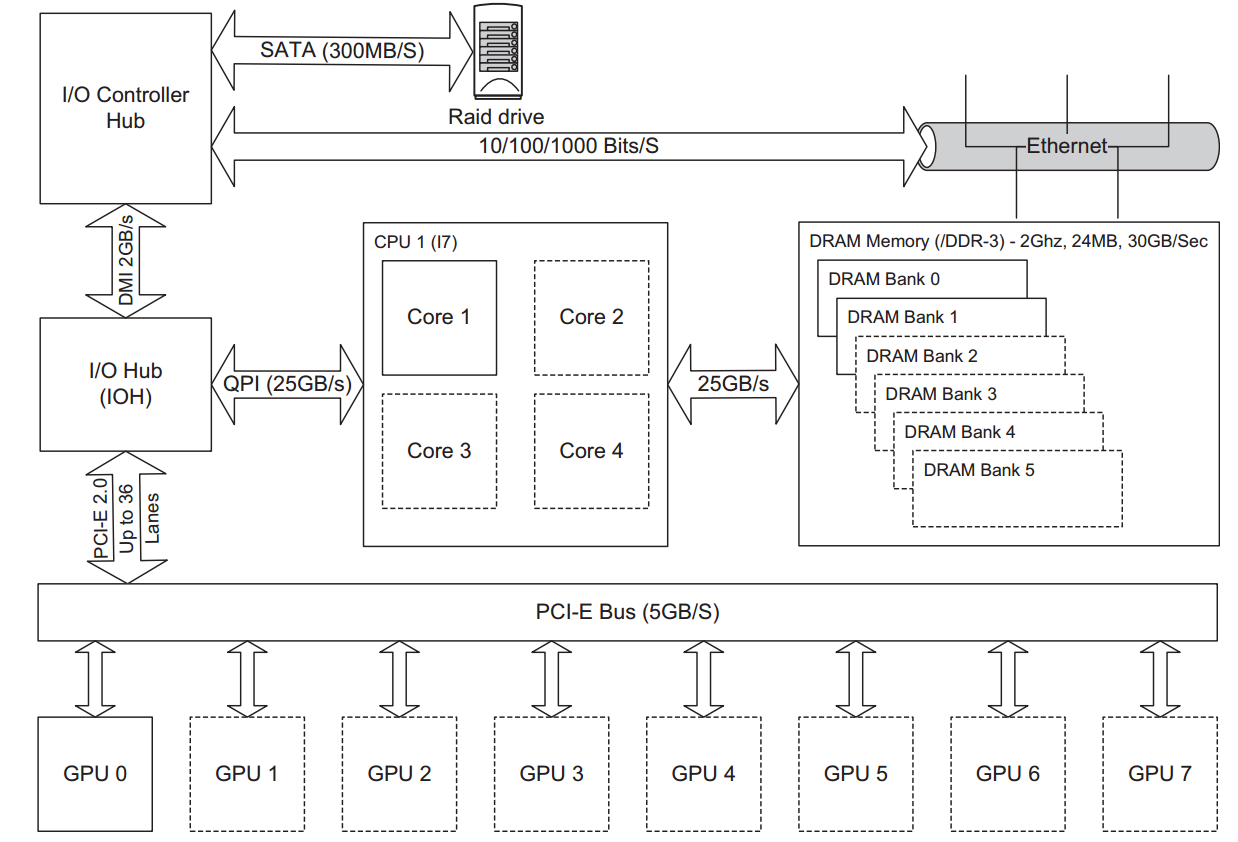
\includegraphics[width=0.7\textwidth]{1_1.PNG}
	\caption{Nehalem/X58 System}
	\label{pl1}
\end{figure}
\begin{figure}[!h]\centering
	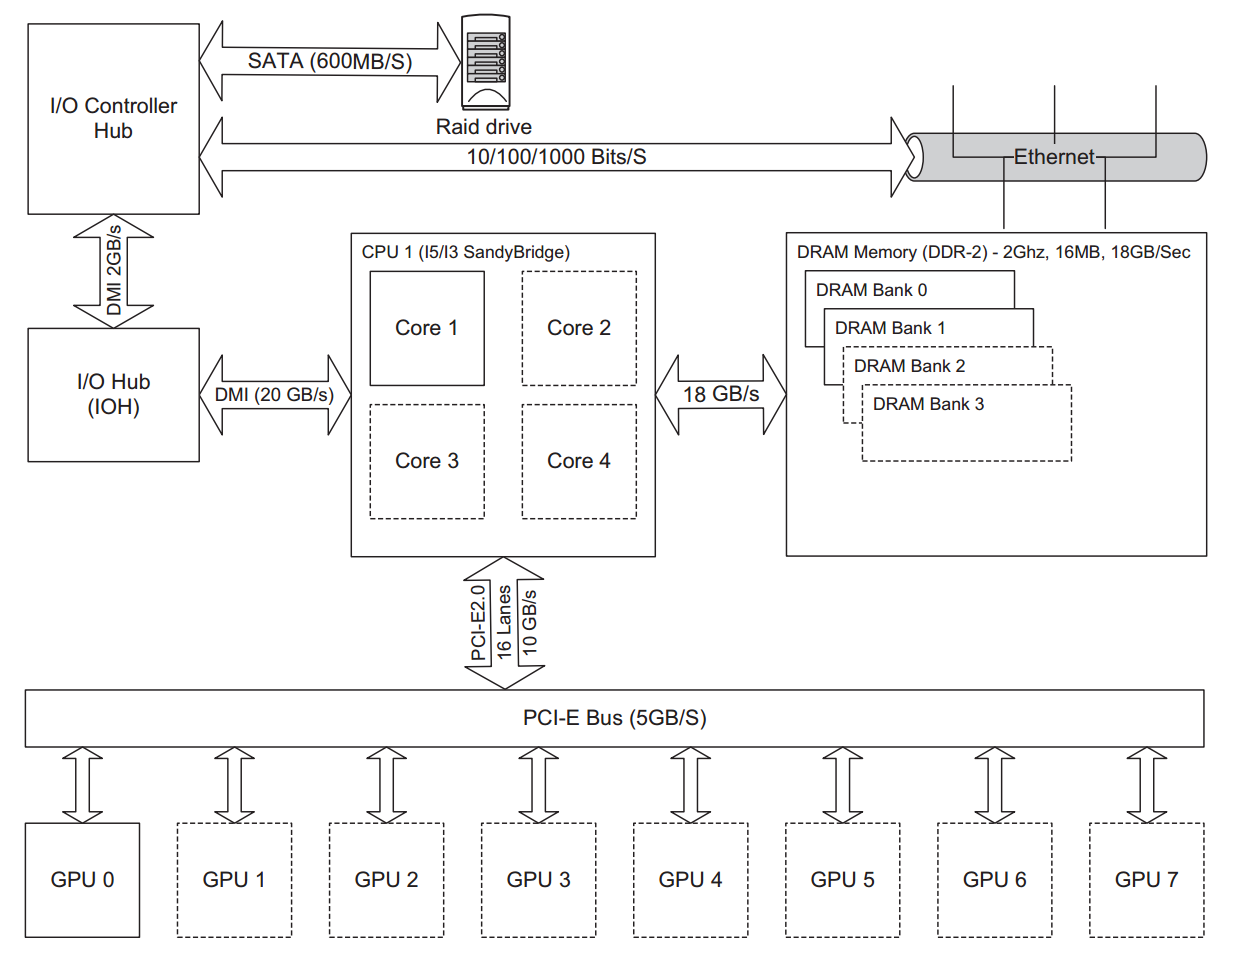
\includegraphics[width=0.7\textwidth]{1_2.PNG}
	\caption{Sandybridge Design}
	\label{pl1}
\end{figure}
\begin{itemize}
	\item \textbf{What is the difference between peripheral connection in these architectures?}

	One of the most noticeable improvements of Sandybridge was the support for the SATA-3 standard, which supports
	600 MB/s transfer rates. This, combined with SSDs, allows for considerable input/output (I/O)
	performance with loading and saving data. While in the Nehalem/X58 architecture peripheral transfer rate is only 300 MB/s. One significant advantage of the AMD chipsets over the Intel ones is the support for up to six SATA
	(Serial ATA) 6 GB/s ports. SATA3 can very
	quickly overload the bandwidth of Southbridge when using multiple SSDs (solid state drives). A PCI-E
	bus solution may be a better one, but it obviously requires additional costs. 
	
	\item \textbf{Does peripheral connection speed matters? Explain.}
	
	 If you consider that the slowest component in any system usually limits the overall throughput, this is something that needs some consideration. For example, SATA3 can very
	 quickly overload the bandwidth of Southbridge when using multiple SSDs (solid state drives). As another fact, If using MPI (Message Passing Interface), which is commonly used in clusters, the latency for this
	 arrangement can be considerable if the Ethernet connections are attached to the Southbridge instead
	 of the PCI-E bus. Consequently, dedicated high-speed interconnects like InfiniBand or 10 Gigabit
	 Ethernet cards are often used on the PCI-E bus.
	 
	\item \textbf{What kind of port is used to connect to the GPU? What are the attributes of this port?}
	
	PCI-E is used. PCI-E (Peripheral Communications Interconnect Express) is an interesting bus as, unlike its
	predecessor, PCI (Peripheral Component Interconnect), it’s based on guaranteed bandwidth. In the
	old PCI system each component could use the full bandwidth of the bus, but only one device at
	a time. Thus, the more cards you added, the less available bandwidth each card would receive. PCI-E
	solved this problem by the introduction of PCI-E lanes. These are high-speed serial links that can be
	combined together to form X1, X2, X4, X8, or X16 links. Most GPUs now use at least the PCI-E
	2.0, X16 specification, as shown in Figure 3.1. With this setup, we have a 5 GB/s full-duplex bus,
	meaning we get the same upload and download speed, at the same time. Thus, we can transfer 5 GB/
	s to the card, while at the same time receiving 5 GB/s from the card. However, this does not mean
	we can transfer 10 GB/s to the card if we’re not receiving any data (i.e., the bandwidth is not
	cumulative).
	
	\item \textbf{According to the given architectures in figure 1.1 and figure 1.2, how many GPUs can be connected in each system? What about their bandwidth? Explain.
	}
	In both cases, 8 GPUs can be connected to the system via PCI-E bus. however, the big downside of socket 1155 Sandybridge design: It supports only 16 PCI-E
	lanes, limiting the PCI-E bandwidth to 16 GB/s theoretical, 10 GB/s actual bandwidth. Thus each GPU is able to use $\frac{10}{8} = 1.25$ GB/s of bandwidth available. On the other hand, the \textit{Nehalem/X58} provides $\frac{16}{8} = 2$ GB/s of bandwidth.
\end{itemize}

\section{GPU Architecture}
Main components of a GPU are given below. Describe each of these components and the relationship between them.
\begin{itemize}
	\item \textbf{Memory  (Global, Constant, Shared)}: CUDA C makes available a region of memory that we call \textbf{shared} memory. This region of memory brings along with it another extension to the C language akin to \_\_device\_\_ and \_\_global\_\_. As a programmer, we can modify our variable declarations with the CUDA C keyword \_\_shared\_\_ to make this variable resident in shared memory. The CUDA C compiler treats variables in shared memory differently than typical variables. It creates a copy of the variable for each block that you launch on the GPU. Every thread in that block shares the memory, but threads cannot see or modify the copy of this variable that is seen within other blocks. This provides an excellent means by which threads within a block can communicate and collaborate on computations. Furthermore, shared memory buffers reside physically on the GPU as opposed to residing in off-chip DRAM. Because of this, the latency to access shared memory tends to be far lower than typical buffers, making shared memory effective as a per-block. However, if your program is using too much shared memory to store data, or your threads simply need to share too much data at once, then it is possible that the shared memory is not big enough to accommodate all the data that needs to be shared among the threads. In such a situation, threads always have the option of writing to and reading from \textbf{global} memory. Global memory is much slower than accessing shared memory; however, global memory is much larger. For most video cards sold today, there is at least 128MB of memory the GPU can access. The CUDA language makes available another kind of memory known as constant memory. As the name may indicate, we use constant memory for data that will not change over the course of a kernel execution. NVIDIA hardware provides 64KB of \textbf{constant} memory that it treats differently than it treats standard global memory. In some situations, using constant memory rather than global memory will reduce the required memory bandwidth.
	
	\item \textbf{Streaming Multiprocessors \& Streaming Processors}: A GPU is an array of SMs. Each of these SMs have N cores. There are number of key components making
	up each SM, however, not all are shown here for reasons of simplicity. The most significant part is that
	there are multiple SPs in each SM. Note that Each SM has a separate bus into the shared memory, constant memory, and global memory
	spaces.
	
	\item \textbf{What is GDDR memory? Explain the differences with a DDR memory? Why not using a DDR in graphics card?} Global memory is supplied via GDDR (Graphic Double Data Rate) on the graphics card. This is
	a high-performance version of DDR (Double Data Rate) memory. Memory bus width can be up to 512 bits
	wide, giving a bandwidth of 5 to 10 times more than found on CPUs, up to 190 GB/s with the Fermi
	hardware. Thus, the main difference between DDR and GDDR is that the \textit{Bandwidth} on GDDR is much higher than DDR memories. That's mainly because of the high number of cores accessing the memory simultaneously.
	
	\item \textbf{Explain the inner components of figure 2.1.} 
	\begin{figure}[!h]\centering
		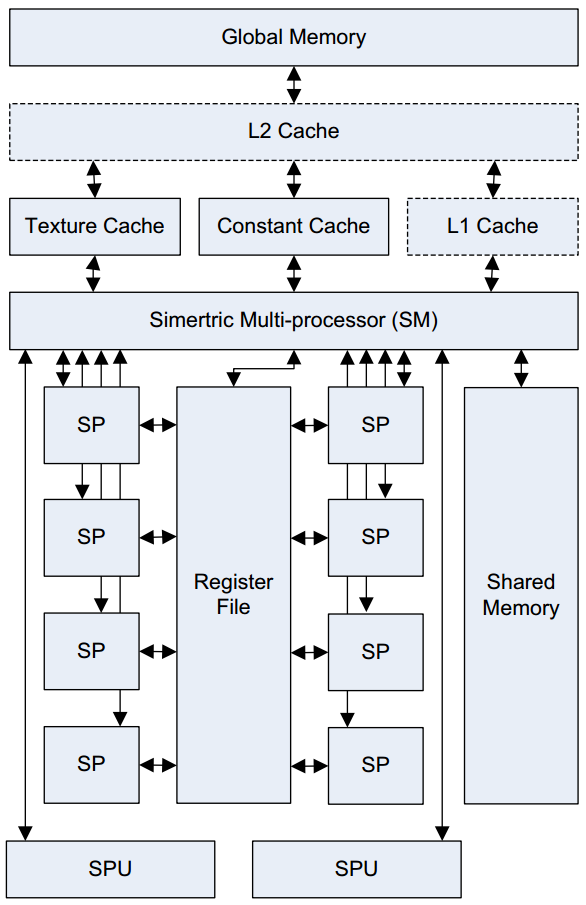
\includegraphics[width=0.45\textwidth]{2_1.PNG}
		\caption{Inside an SM}
		\label{pl1}
	\end{figure}
	The very first component is the Global Memory which is called GDDR in graphics processing unit. There are also 2 levels of cache in a GPU. The first layer cache is divided into three types called \textit{Texture Cache, Constant Cache and L1 Cache}. Each GPU Consists of multiple SMs that they contain some Streaming Processors (A.K.A Cores). Each of these SPs have their own registers in a huge register file. Each SM also has two or more special-purpose units (SPUs), which perform special hardware
	instructions, such as the high-speed 24-bit sin/cosine/exponent operations. Double-precision units are
	also present on GT200 and Fermi hardware.
	
	\item \textbf{What are the differences between \textit{Texture, Global and Constant} memories?} Texture memory is a special view onto the global memory, which is useful for data where there is interpolation, for example, with 2D or 3D lookup tables. It has a special feature of
	hardware-based interpolation. Constant memory is used for read-only data and is cached on all
	hardware revisions. Like texture memory, constant memory is simply a view into the main global
	memory.
	Global memory is supplied via GDDR (Graphic Double Data Rate) on the graphics card. This is
	a high-performance version of DDR (Double Data Rate) memory. Memory bus width can be up to 512 bits
	wide, giving a bandwidth of 5 to 10 times more than found on CPUs, up to 190 GB/s with the Fermi
	hardware. They are physically identical but, the addressing sections of each is different from the other one.
\end{itemize}

\section{Compute Capability}
The \textit{compute capability} of a device is represented by a version number, also sometimes
called its "SM version". This version number identifies the features supported by the
GPU hardware and is used by applications at runtime to determine which hardware
features and/or instructions are available on the present GPU.
The compute capability comprises a major revision number X and a minor revision
number Y and is denoted by X.Y.
Devices with the same major revision number are of the same core architecture. The
major revision number is 5 for devices based on the Maxwell architecture, 3 for devices
based on the Kepler architecture, 2 for devices based on the Fermi architecture, and 1 for
devices based on the Tesla architecture.
The minor revision number corresponds to an incremental improvement to the core
architecture, possibly including new features.
\section{Occupancy in CUDA}
Represents that how much of the threads in an streaming multiprocessor are occupied during a process. It can be computed using the following formula:
\begin{equation}
	OCC = \frac{Threads\ in\ SM}{Max\ Threads\ in\ SM}
\end{equation}
Occupancy subjects to various constraints:
\begin{itemize}
	\item Completed blocks assigned to each SM.
	\item If combined register usage exceeds SM limits then we'll have to limit the number of blocks in an SM.
	\item If combined shared memory usage exceeds SM limits then we'll have to limit the number of blocks in an SM.
\end{itemize}

\section{Vector Addition Indexing}
Suppose we want to add two vectors together. Find the proper index for the output vector in case we want each thread to compute a single component of the vector.
$$
	i = blockIdx.x*blockDim.x + threadIdx.x; 
$$

\section{Vector Addition Grid}
Suppose two vectors with 8000 elements. We want each thread to compute one of these elements and the block size of the threads is 1024. Programmer adjusts the \textit{Kernel Launch} so that the minimum blocks of threads are used. Find the number of threads in a grid in this case. 

There will be obviously 8192 threads in the grid while 192 of them are doing nothing.
\end{document}